\section{Experimental Results}
\begin{frame}{Experimental Results}
\begin{itemize}
    \item \textbf{Tasks}
    \begin{itemize}
        \item A range of continuous control tasks from the OpenAI gym benchmark suite
        \item RL-Lab implementation of the Humanoid task
        \item The easier tasks can be solved by a wide range of different algorithms, the more complex benchmarks, such as the 21-dimensional Humanoid (rllab) are exceptionally difficult to solve with off-policy algorithms.
    \end{itemize}
    \item \textbf{Baselines:}
    \begin{itemize}
        \item DDPG, SQL, PPO, TD3 (concurrent)
        \item TD3 is an extension to DDPG that first applied the double Q-learning trick to continuous control along with other improvements.
    \end{itemize}
\end{itemize}
\end{frame}
\begin{frame}{SAC: Results}
\begin{figure}
    \centering
    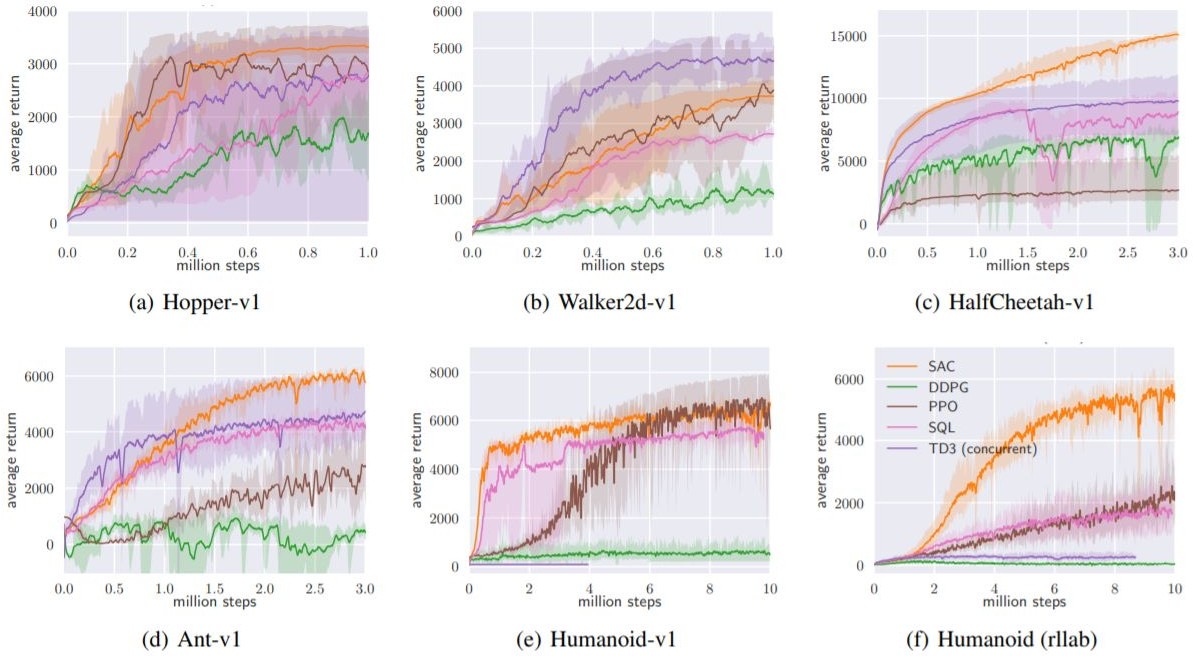
\includegraphics[width=\textwidth,height=0.85\textheight,keepaspectratio]{images/soft-actor-critic/figures/sac-results-grid.jpg}
\end{figure}
\end{frame}
\begin{frame}{Experimental Results: Ablation Study}
\begin{columns}[T]
\begin{column}{0.45\textwidth}
\vspace{1em}
\begin{itemize}
    \item How does the stochasticity of the policy and entropy maximization affect the performance?
    \vspace{0.5em}
    \item Comparison with a deterministic variant of SAC that does not maximize the entropy and that closely resembles DDPG
\end{itemize}
\end{column}
\begin{column}{0.5\textwidth}
\begin{figure}
    \centering
    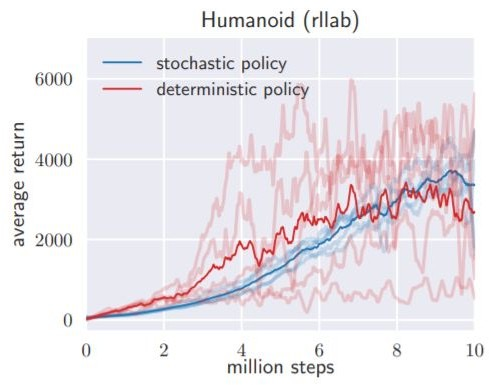
\includegraphics[width=\linewidth,height=0.7\textheight,keepaspectratio]{images/soft-actor-critic/figures/sac-ablation.jpg}
\end{figure}
\end{column}
\end{columns}
\begin{flushright}
    \tiny\url{https://arxiv.org/abs/1801.01290}
\end{flushright}
\end{frame}
\begin{frame}{Experimental Results: Hyperparameter Sensitivity}
\begin{figure}
    \centering
    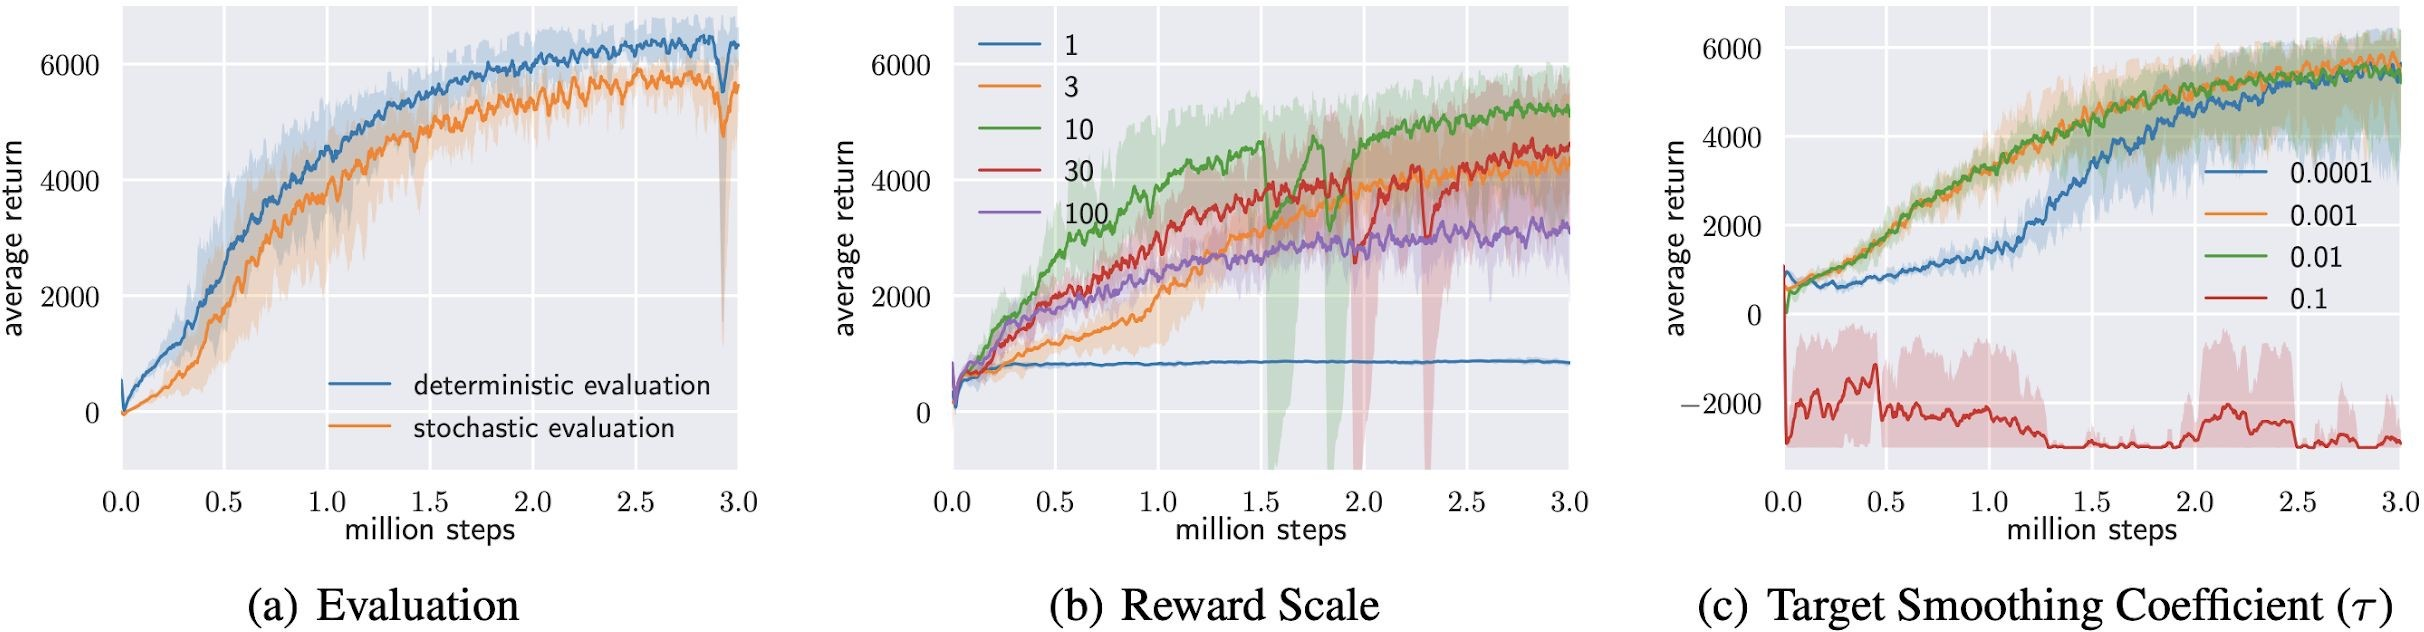
\includegraphics[width=\textwidth,height=0.8\textheight,keepaspectratio]{images/soft-actor-critic/figures/sac-hyperparam.jpg}
\end{figure}
\begin{flushright}
    \tiny\url{https://arxiv.org/abs/1801.01290}
\end{flushright}
\end{frame}
